\documentclass[letterpaper, 10 pt, conference]{ieeeconf}  % Comment this line out if you need a4paper
%\documentclass[a4paper, 10pt, conference]{ieeeconf}      % Use this line for a4 paper
\IEEEoverridecommandlockouts                              % This command is only needed if 
                                                          % you want to use the \thanks command

\overrideIEEEmargins                                      % Needed to meet printer requirements.

%In case you encounter the following error:
%Error 1010 The PDF file may be corrupt (unable to open PDF file) OR
%Error 1000 An error occurred while parsing a contents stream. Unable to analyze the PDF file.
%This is a known problem with pdfLaTeX conversion filter. The file cannot be opened with acrobat reader
%Please use one of the alternatives below to circumvent this error by uncommenting one or the other
%\pdfobjcompresslevel=0
%\pdfminorversion=4

% See the \addtolength command later in the file to balance the column lengths
% on the last page of the document

% The following packages can be found on http:\\www.ctan.org
%\usepackage{graphics} % for pdf, bitmapped graphics files
%\usepackage{epsfig} % for postscript graphics files
%\usepackage{mathptmx} % assumes new font selection scheme installed
%\usepackage{times} % assumes new font selection scheme installed
\usepackage{amsmath} % assumes amsmath package installed
%\usepackage{amssymb}  % assumes amsmath package installed
\usepackage{subfig}
\usepackage{graphicx}
\usepackage{bm}
\usepackage{xcolor}
\makeatletter
\newcommand{\rom}[1]{\uppercase\expandafter{\romannumeral #1\relax}}

\title{\LARGE \bf
%Fusion of IMU and Flowdeck Sensors for \\Emergency Landing of Quadrotors
State Estimation of Quadrotors with Bias Correction \\ for Emergency Landing
}






\author{Sasan Vakili and Wenda Zhao% <-this % stops a space
\thanks{The authors are with the Dynamic Systems Lab (www.dynsyslab.org) at
the University of Toronto Institute for Aerospace Studies (UTIAS), Canada.
Email: sasan.vakili@mail.utoronto.ca, wenda.zhao@mail.utoronto.ca}%
}


\begin{document}



\maketitle
\thispagestyle{empty}
\pagestyle{empty}


%%%%%%%%%%%%%%%%%%%%%%%%%%%%%%%%%%%%%%%%%%%%%%%%%%%%%%%%%%%%%%%%%%%%%%%%%%%%%%%%
\begin{abstract}

In this paper, we present an approach, based on the well-known Extended Kalman Filter, to estimate the quadrotor's states fusing data from the onboard sensors. This estimation will provide accurate states for the quadrotor to generate safe landing trajectory in emergency situations. The presented approach is simulated based on real dataset from experiments of a Crazyflie platform. Observability analysis is provided in this paper to reveal the theoretical limitation of this estimator due to sensor constrains. Sensor biases are considered in the estimator, which provides decent improvements in the estimation results.
\end{abstract}


%%%%%%%%%%%%%%%%%%%%%%%%%%%%%%%%%%%%%%%%%%%%%%%%%%%%%%%%%%%%%%%%%%%%%%%%%%%%%%%%
\section{Introduction} 

Complex and challenging tasks are performed via Unmanned Aerial Vehicles (UAVs or quadrotors) in various industrial fields. Quadrotors have been used for various applications such as terrain surveying and monitoring~\cite{bamford-fragblast12}, precision agriculture~\cite{gonzalez2013using}, robotic swarm performance~\cite{li2017learning}, and many others. The increasing application of quadrotors in high-risk and challenging environments requires various techniques to guarantee their safety (\cite{berkenkamp2016safe},~\cite{warren2018there}). The current autonomous quadrotor systems are considerably dependent on the communication between quadrotors and a ground station. The purpose of this communication is to receive a control command, which is provided by heavy computational algorithm running on the ground station systems~\cite{luis2018trajectory},~\cite{du2018fast}. However, there are risks in case
of communication loss. Communication loss between the ground station and a quadrotor will lead to loss of
localization information and control commands; hence, crash of the quadrotor. In order to avoid such scenarios, a simplified version of localization and control algorithm should be implemented onboard to perform safe landing in emergency situations. In this paper, we focus on the first required step for this algorithm: estimation of a quadrotor's position, velocity and orientation states only using onboard sensors.

State estimation on mobile robots has been widely investigated in order to perform highly autonomous and robust tasks~\cite{bloesch2013state},~\cite{mueller2016covariance}. In many indoor localization scenarios, researchers fuse different types of sensor data to achieve accurate state estimation results. Onboard vision systems, such as stereo-vision systems and optical flow cameras, are often used to measure the relative movement of quadrotors~\cite{landry2015planning}. A relatively new radio measurement sensor ultra-wideband (UWB)~\cite{preiss2017crazyswarm},~\cite{ledergerber2017ultra} are used to provide global localization information. Fusing UWB range sensor data together with onboard camera measurements has been demonstrated accurate estimation results in~\cite{Mueller2015FusingUR}. Aside from position, velocity and orientation states, there are works such as~\cite{mckinnon2016unscented} estimating the external force and torque acted on quadrotors in order to design robust controller for flying in challenging environments.

\begin{figure}[t]
\centering
	%\subfloat[Crazyflie 2.0]{\label{a}
	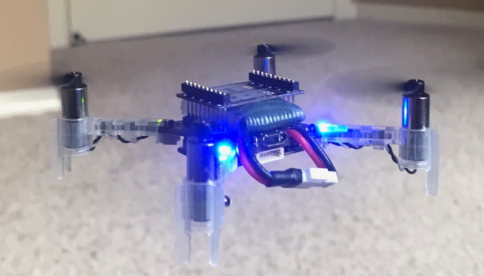
\includegraphics[width=3in]{curve/Drone.png}   \\
	%\subfloat[Experimental platform]{\label{b}
	\includegraphics[width=3in]{curve/Vicon.jpg}%}  \\
%\centering
\caption{Nano-quadrotor: Crazyflie 2.0 with IMU and onboard flow deck sensor. Experimental platform is in Dynamic Systems Lab.}
\label{DSL}
\end{figure}

The goal of this paper is to present an approach to estimate a quadrotor's position, velocity and orientation states when the communication with ground station fails. Dataset is built based on a nano-quadrotor experiment platform in Dynamic Systems Lab (Fig.~\ref{DSL}). We implement an Extended Kalman Filter to fuse the onboard sensor data and estimate the quadrotor's states. We compare the estimation results with different measurement models and analyze the effects of sensor bias and the limitation of system observability.  

The structure of this paper is as follows: the problem is formulated in section \rom{2}. Section \rom{3} discusses the onboard sensor models used in this paper and section \rom{4} presents the main body of the Extended Kalman Filter with two different measurement models. Observability is analyzed in section \rom{5} which reveals the fundamental limitation of our estimator and the bias estimation methods are provided to improve the estimator's performance. The estimation results are compared and presented in section \rom{6} and future works are discussed in \rom{7}. 


\section{Problem Statement}   
The goal of this work is to estimate the full state of the quadrotor based on the onboard sensors in order to provide accurate states information for safe landing. We collect the sensor data from the Crazyflie 2.0 quadrotor and estimate the full state based on the real dataset. 
\subsection{Quadrotor Dynamics}
The Crazyflie 2.0 quadrotor is modelled as a rigid body, with double integrator dynamics. This is a simplified dynamic model of a quadrotor equipped with an underlying position controller. We use $\bm{p}_k$,$\bm{v}_k$ and $\bm{a_k}$ to represent the discretized position, velocity and accelerations of the quadrotor at time step $k$ with accelerations treated as inputs. With a discretization time step $\Delta t$, the dynamic equations are given by
\begin{equation}
\begin{split}
\bm{p}_{k+1}&=\bm{p}_{k}+\Delta t\bm{v}_k +\frac{\Delta t^2}{2}\bm{a}_k   \\
\bm{v}_{k+1}&=\bm{v}_{k}+\Delta t \bm{a}_k
\end{split}
\end{equation}  
\subsection{Measurement Limitation}
In this problem, there are only two sensors available: IMU and flow deck. Due to the limitation of sensor data, we perform two different types of measurement models for the estimator, compare the performance and analyze the observability of the system in later sections.
\subsection{Full State Estimation}
The focus of this work is on estimating the position $\bm{p}=(x,y,z)$ and velocity $\bm{v}=(v_x,v_y,v_z)$ of the quadrotor in inertial coordinate frame at each time step for collision-free purpose. Since quadrotor's motion model contains rotation matrix $\bm{C}$, we also need to estimate the orientation of the quadrotor at each time step. In this paper, we express the angular dependence and estimate the orientation of the quadrotor by means of quaternions using the Newton-Euler equations $\bm{q}=(q_0,q_1,q_2,q_3)=[q_0,\bm{q}_v]^T$. Therefore, the full state of the quadrotor contains position, velocity and orientation. The biases on acceleration and angular velocity achieved from IMU sensor are also added into the state vector in order to estimate them and eliminate their effect on the desired states of the system.

\section{Sensor Models}   
This section discusses the sensor models used in this work. The particular model choices represent a trade-off between simplicity and accuracy. Process and measurement noise will be modelled as zero-mean Gaussian distribution in this paper. By increasing the corresponding covariance matrix, we can handle this inaccurate assumption and achieve reasonable sensor data.
\subsection{Inertial Sensor}
The inertial IMU sensor measures the proper acceleration $\bm{f}$ and the angular rate $\bm{\omega}$ of the quadrotor. The proper acceleration is related to the absolute acceleration $\bm{a}$ by
\begin{equation}
\bm{f}=\bm{C}\left(\bm{a}+\bm{g}\right)
\end{equation}
where $\bm{C}$ is the matrix rotating coordinates of a vector expressed in the inertial coordinate frame $\bm{I}$ into the body coordinate frame $\bm{B}$. The IMU quantities $\bm{f}$ and $\bm{\omega}$ are assumed to be directly measured in the body coordinate frame $\bm{B}$. 
\begin{equation}
	\bm{f} = \bm{\tilde{f}}+\bm{w}_f
\end{equation}
\begin{equation}
	\bm{\omega} = \bm{\tilde{\omega}}+\bm{w}_{\omega}
\end{equation}
The measured quantities $\bm{f}$ and $\bm{\omega}$ are assumed to be affected by zero-mean Gaussian noise $\bm{w}_f$ and $\bm{w}_{\omega}$. The noise terms are simulated by the corresponding covariance parameters $\bm{Q}_f$ and $\bm{Q}_{\omega}$. For simplicity, the noise are modelled by independent Gaussian distribution and each covariance parameter is a diagonal matrix. 
\subsection{Flowdeck Sensor}
The onboard flowdeck sensor contains a \textit{vl53l0x} ToF sensor measuring the distance to the ground and a \textit{PMW3901} optical flow sensor measuring the movements related to the ground. The ToF range sensor provides centimetre precision measurements at a range of $h<1.2-2~[m]$ depending on the mode of operation and the properties of the reflective surface. The angle of aperture of the collector is $\theta_{pz}=25^{\circ}$ and the distribution of the measurement error was experimentally shown to be well approximated by a zero-mean Gaussian distribution with variance $Q_z$~\cite{greiff2017modelling}. The measured range distance $z$ in quadrotor's body coordinate frame is modeled by
\begin{equation}
	z=\tilde{z}+w_z
\end{equation}
where $w_z\sim\mathcal N(0,Q_z)$ indicates the measurement noise of ToF range sensor.

For onboard optical flow sensor measurements, we presume to know the aperture angle of the camera $\left(\theta_{px},\theta_{py}\right)~[rad]$ and the numbers of pixels $\left(N_x,N_y\right)~[pixels]$ of the image which is tracked in time. Then the optical flow method measures the accumulated pixel count $\left(\Delta n_x,\Delta n_y\right)~[pixels/s]$ at small time steps $\Delta t~[s]$. Let $\left(\theta_x,\theta_y\right)$ denote the angular offset about the $x_B$ and $y_B$ axis in body frame.
\begin{equation}
\theta_x=\frac{\theta_{px}}{N_y}n_y, \theta_y=\frac{\theta_{py}}{N_x}n_x
\end{equation}
Then quadrotor's velocities $v_x$ and $v_y$ in body coordinate frame can be computed by the approximated model below.
\begin{equation}
v_x=h\frac{\theta_y}{\Delta t}=h\frac{\theta_{py}}{\Delta tN_x}\Delta n_x + w_{v_x}
\end{equation}
\begin{equation}
v_y=h\frac{\theta_x}{\Delta t}=h\frac{\theta_{px}}{\Delta tN_y}\Delta n_y + w_{v_y}
\end{equation}
Where $h$ is the height in inertial frame and the measurement noises are modelled by zero-mean Gaussian noise $w_{v_x}$ and $w_{v_y}$.
\begin{equation}
h=\left \{
  \begin{split}
    	&~~~~~~~~~~z &if ~~|\alpha|<\theta_{pz}/2     \\                 
 	 &\frac{z}{cos(|\alpha|-\theta_{pz}/2)} &if ~~|\alpha|\geq\theta_{pz}/2 
  \end{split}
\right.  
\end{equation}
\begin{equation}
\alpha=arccos\left(cos(\phi)cos(\theta)\right)
\end{equation}
Where $z$ is the measurement data from ToF range sensor and $\alpha$ is the overall filtered angle.

\section{State Estimation}  
In this section, we present our approach for the quadrotor's full state estimation. As mentioned in previous sections, an Extended Kalman Filter is built to fuse IMU and flow deck sensor data and estimate the quadrotor's position, velocity and orientation at each time step. The following paragraph starts by defining the state vector of the filter and subsequently continues by formulating the filter models and relative equations.   

\subsection{Filter State Definition} 

The state vector of the filter should be chosen in advance such that the corresponding prediction and measurement equations can be expressed in a clean and consistent manner. We use quaternions $\bm{q}$ as our states, representing the rotation from the inertial coordinate frame $I$ to the body coordinate frame $B$. In the setting, we are inspired by the work done by~\cite{bloesch2013state}. Quaternions have two important properties: they are singularity-free and less susceptible to round-off errors than rotation matrices. 
Together with position $\bm{p}$ and velocity $\bm{v}$ in the body coordinate frame, we have the state vector:
\begin{equation}
\bm{x}:=\left(x,y,z,v_x,v_y,v_z,q_0,q_1,q_2,q_3\right)
\end{equation}
 
The presented Extended Kalman Filter represents the uncertainties of the estimated state vector via the covariance matrix $\bm{P}$ of the corresponding state error vector $\delta x$. 
\begin{equation}
\begin{split}
\bm{P} &:= Cov(\bm{\delta x})  \\
\bm{\delta x} &:=\left(\delta x,\delta y,\delta z,\delta v_x,\delta v_y,\delta v_z,\delta \bm{q}\right)
\end{split}
\end{equation}

Since the orientation state $\bm{q}$ possesses 3 degrees of freedom, its covariance term should therefore be represented by a 3 dimensional covariance matrix. The error of the pose is then represented as a 3-dimensional rotation vector $\bm{\delta \phi}$. There exists a map $\zeta(\cdot)$ relating the error rotation vector to the quaternion error.
\begin{equation}
\bm{\delta q} = \zeta(\bm{\delta \phi})
\end{equation}
\begin{equation}
\renewcommand\arraystretch{1.7}
 \zeta(v)=\begin{bmatrix}
  sin\left(\frac{1}{2}\|v\|\right)\frac{v}{\|v\|}  \\
  cos\left(\frac{1}{2}\|v\|\right)
 \end{bmatrix}
\end{equation} 
Then the quaternion $\bm{q}$ can be updated based on the relation
\begin{equation}
\bm{q}=\bm{\delta q}\otimes \bm{\hat{q}}
\end{equation}
where $\bm{\hat{q}}$ indicates the previous estimated quaternion value and $\otimes$ is the quaternion multiplication operator.
 
Given a quaternion at each time step, the corresponding rotation matrix $C$ can be determined.
\begin{equation}
\bm{q} =\begin{bmatrix}
q_0  \\
q_1  \\
q_2  \\
q_3  
\end{bmatrix}=\begin{bmatrix}
q_0  \\
\bm{q}_v
\end{bmatrix}   
\end{equation}
\begin{equation}
\bm{C} = (2q_0^2-1)\bm{1}_{3\times3}+2\bm{q}_v\bm{q}_v^T-2q_0\bm{q}_v^{\times}
\end{equation}

Each time we estimate the rotation vector $\bm{\delta \phi}$, update the quaternion state $\bm{q}$ and convert back to rotation matrix $\bm{C}$ for the computation of model and observation models.    

\subsection{Prediction Model}
The prediction equations are responsible for propagating the state from one time step to the next. IMU measurements $\bm{f}$ and $\bm{\omega}$ are treated as the input. The continuous time differential equations of the motion model can be formulated:
\begin{equation}
\begin{split}
\bm{\dot{p}} &= \bm{v}   \\
\bm{\dot{v}} &= \bm{a} =\bm{C}^T\bm{f}-\bm{g} = \bm{C}^T(\bm{\tilde{f}}-\bm{w}_f)-\bm{g}  \\
\bm{\dot{q}} &=\frac{1}{2}\bm{\Omega}\bm{\omega}\bm{q}   =\frac{1}{2}\bm{\Omega}(\bm{\tilde{\omega}}-\bm{w}_{\omega})\bm{q}  
\end{split}
\end{equation} 
where $\bm{\Omega}(\cdot)$ maps an arbitrary rotational rate $\omega$ to the $4\times 4$ matrix used for representing the corresponding quaternion rate:
\begin{equation}
\bm{\Omega}:~\omega\rightarrow \bm{\Omega}(\omega)=\begin{bmatrix}
0  			&\omega_z  		 &-\omega_y  	 &\omega_x  \\
-\omega_z   &0               & \omega_x      &\omega_y  \\
\omega_y    &-\omega_x       & 0             &\omega_z  \\
-\omega_x   &-\omega_y       &-\omega_z      &  0
\end{bmatrix}
\end{equation}
The process noise of position, velocity and orientation are modelled by independent zero-mean Gaussian distribution. The variance matrix $\bm{Q}$ is 
\begin{equation}
\renewcommand\arraystretch{1.3}
\bm{Q}=\begin{bmatrix}
\bm{\delta^2_p}     &0              	 &0    \\
0              		&\bm{\delta^2_v}     &0    \\
0              		&0              	 &\bm{\delta^2_o}   
\end{bmatrix}
\end{equation}
where $\bm{\delta^2_p}$ is the variance of position noise, $\bm{\delta^2_v}$ is the variance of velocity noise and $\bm{\delta^2_q}$ is the variance of orientation noise. The dimension of $\bm{Q}$ is therefore $9\times 9$. 
\subsection{Measurement Model}
Due to the limitation of onboard sensor, we can only get the measurements of velocities in $x$ and $y$ directions $(v_x,v_y)$ and measurement of position in $z$ direction. All three measurements are in quadrotor's body frame. In this work, we provide two different measurement models by processing the sensor data and perform two ways of correction in the Extended Kalman Filter.
\subsubsection{Measurement Model \rom{1}}
For the first measurement model, we integrate the velocities in $x$ and $y$ directions and get the position measurements in $x$ and $y$ directions. The equations in discretization time steps can be expressed as
\begin{equation}
\begin{split}
x_{k+1} &= v_{xk} \Delta t+x_k   \\
y_{k+1} &= v_{yk} \Delta t+y_k
\end{split}
\end{equation} 
where $x_{k+1}$ and $y_{k+1}$ are the position measurements at time step $k+1$ in quadrotor's body coordinate frame.

The first measurement model is
\begin{equation}
\renewcommand\arraystretch{1.2}
y=\begin{bmatrix}
\tilde{x}   \\
\tilde{y}   \\
\tilde{z}   \\
\end{bmatrix}=\begin{bmatrix}
\bm{C} & \bm{0}_{3\times 3}  
\end{bmatrix}\begin{bmatrix}
	x   \\
	y   \\
	z   \\
	v_x   \\
	v_y   \\
	v_z   
\end{bmatrix}+\begin{bmatrix}
n_{px}   \\
n_{py}   \\
n_{pz}
\end{bmatrix}
\end{equation}
where $\tilde{x},\tilde{y},\tilde{z}$ are position measurements in body coordinate frame and $n_{px},n_{py},n_{pz}$ are the corresponding measurement noise. 

The measurement noises are modelled as independent zero-mean Gaussian distribution with covariance matrix $\bm{R_p}$:
\begin{equation}
\renewcommand\arraystretch{1.2}
\bm{R_p} = \begin{bmatrix}
R_{x}  & 0   & 0 \\
0  & R_{y}   & 0 \\
0  & 0   & R_{z} 
\end{bmatrix}
\end{equation}

\subsubsection{Measurement Model \rom{2}}
For the second measurement model, we take the derivative of the $z$ position measurement and get the velocity $v_z$ in $z$ directions. The equations in discretization time steps can be expressed as
\begin{equation}
v_{z(k+1)} = \frac{z_{k+1}-z_{k}}{\Delta t} 
\end{equation} 
where $v_{z(k+1)}$ is the velocity measurement at time step $k+1$ in quadrotor's body coordinate frame.

The second measurement model is
\begin{equation}
\renewcommand\arraystretch{1.2}
y=\begin{bmatrix}
\tilde{v}_x   \\
\tilde{v}_y   \\
\tilde{v}_z   \\
\end{bmatrix}=\begin{bmatrix}
\bm{0}_{3\times 3} & \bm{C}
\end{bmatrix}\begin{bmatrix}
	x   \\
	y   \\
	z   \\
	v_x   \\
	v_y   \\
	v_z   
\end{bmatrix}+\begin{bmatrix}
n_{vx}   \\
n_{vy}   \\
n_{vz}
\end{bmatrix}
\end{equation}
where $(\tilde{v_x},\tilde{v_y},\tilde{v_z})$ are the velocity measurements in body frame and $n_{vx},n_{vy},n_{vz}$ are the corresponding measurement noises. 

The measurement noises are modelled as independent zero-mean Gaussian distribution with covariance matrix $\bm{R_v}$:
\begin{equation}
\renewcommand\arraystretch{1.2}
\bm{R_v} = \begin{bmatrix}
R_{vx}  & 0   & 0 \\
0  & R_{vy}   & 0 \\
0  & 0   & R_{vz} 
\end{bmatrix}
\end{equation}

\subsection{Extened Kalman Filter Equations}
The following equation is introduced in order to linearize and calculate the Jacobian matrices of the prediction and measurement models. 
\begin{equation}
\Gamma_n:=\sum_{i=0}^{\infty}\frac{\Delta t^{i+n}}{\left(i+n\right)!}\omega^{\times i}
\end{equation}
where the $\left(\cdot\right)^{\times}$ is the skew-symmetric matrix operator. This exponential map connects the matrix exponential to series expansion. For $n=0$ it provides:
\begin{equation}
\Gamma_0=\sum_{i=0}^{\infty}\frac{\left(\Delta t\omega^{\times}\right)^i}{i!}=exp(\Delta t\omega^{\times})
\end{equation}

$\Gamma_0$ represents the incremental rotation matrix if rotating an arbitrary coordinate frame with a rotational rate of $-\omega$ for $\Delta t$ seconds.
\subsubsection{Prediction Step}
The Extended Kalman Filter is implemented in a standard way. 
In the prediction step of Extended Kalman Filter, \textit{a posteriori} state  $\bm{\hat{x}_k}$ at time step $k$ is used in the prediction model in order to achieve \textit{a priori} state $\bm{\check{x}_{k+1}}$ at time step $k+1$. The equations can be discretized to:
\begin{equation}
\begin{split}
\bm{\check{x}_{k+1}} &= \bm{\hat{x}_{k}+}\Delta t\bm{\hat{v}_{k}}+\frac{1}{2}\Delta t^2\left(\bm{\hat{C}_{k}}^T \bm{f_k}-e_3g\right) \\
\bm{\check{v}_{k+1}}  &= \bm{\hat{v}_k}+\Delta t\left(\bm{\hat{C}_k}^T \bm{f_k}-e_3 g\right) \\
\bm{\check{q}_{k+1}} &= \zeta\left(\Delta t \bm{\hat{w}_k}\right)\otimes \bm{\hat{q}_{k}}
\end{split}
\end{equation}
where $e_3=(0,0,1)^T$ and $g$ is the acceleration of gravity.
 
Linearizing the system's dynamic motion model, we can compute the Jacobian matrix $\bm{F_k}$. 
\begin{equation}
\renewcommand\arraystretch{1.7}
\bm{F_k}=\begin{bmatrix}
 I   & \Delta tI & -\frac{1}{2} \Delta t^2 \hat{C}_{k-1}^T f_k^{\times}   \\
 0   & I         & -\Delta t \hat{C}_{k-1}^T f_k^{\times}   \\
 0   & 0         & \hat{\Gamma}^T_{0,k}
\end{bmatrix}
\end{equation}

and the the process noise covariance matrix for the linearized model $\bm{Q'}_k$ is:
\begin{equation}
\renewcommand\arraystretch{1.7}
\bm{Q_k'} = \begin{bmatrix}
\frac{\Delta t^3}{3} \bm{Q_f}   & \frac{\Delta t^2}{2} \bm{Q_f}  &0 \\
\frac{\Delta t^2}{2} \bm{Q_f}   & \Delta t \bm{Q_f}              &0 \\
0                           &  0                & \Delta t\bm{Q_w}    
\end{bmatrix}
\end{equation}
where $\bm{Q_f}$ is the variance matrix of acceleration data and $\bm{Q_w}$ is the variance matrix of gyroscope data.

The prediction step Extended Kalman Filter equations are:
\begin{equation}
\begin{split}
\check{P}_k &= F_{k-1}\hat{P}_{k-1}F_{k-1}^T+Q_k'  \\
\check{x}_k &= f(\hat{x}_{k-1},v_k,0)
\end{split}
\end{equation}
where $v_k$ is the input data at time step $k$ and $f(\cdot)$ is the prediction model.
\subsubsection{Correction Step \rom{1}}
We use position measurements $(x,y,z)$ based on the first measurement model for the correction step. Linearizing the measurement model and computing the Jacobian matrix $\bm{G}$, we will have:
\begin{equation}
\bm{G}=\frac{\partial y}{\partial x}=\begin{bmatrix}
-\bm{\check{C}_k}  & \bm{0}_{3\times 3} & (\bm{\check{C}_k}(x, y ,z)^T)^{\times} 
\end{bmatrix}
\end{equation} 

However, this linearization doesn't affect the variance of the measurements and matrix $\bm{R'}$ is:
\begin{equation}
\renewcommand\arraystretch{1.3}
\bm{R'}=\begin{bmatrix}
R_{x}  & 0   & 0 \\
0  & R_{y}   & 0 \\
0  & 0   & R_{z} 
\end{bmatrix}
\end{equation}

\subsubsection{Correction Step \rom{2}}
For the second measurement model, we use velocity measurements $(v_x,v_y,v_z)$ for correction step. Linearize the measurement model and compute the Jacobian matrix $\bm{G}$.
\begin{equation}
\bm{G}=\frac{\partial y}{\partial x}=\begin{bmatrix}
\bm{0}_{3\times 3} & -\bm{\check{C}_k}  &(\bm{\check{C}_k}(v_x,v_y,v_z)^T)^{\times} 
\end{bmatrix}
\end{equation} 

The linearized variance matrix $\bm{R'}$ is:
\begin{equation}
\renewcommand\arraystretch{1.3}
\bm{R'}=\begin{bmatrix}
R_{vx}  & 0   & 0 \\
0  & R_{vy}   & 0 \\
0  & 0   & R_{vz} 
\end{bmatrix}
\end{equation}
\subsubsection{Update States}
Finally, the Jacobian matrix $\bm{G}$ and $\bm{R'}$ are used to correct and update the \textit{a priori} states $\bm{\check{x}}$ from last time step and get the \textit{a posterior} states $\bm{\hat{x}}$. The Extended Kalman Filter equations for the update step are:
\begin{equation}
\renewcommand\arraystretch{1.3}
\begin{split}
&K_k = \check{P}_k G_k^T\left(G_k\check{P}_k G_k^T + R_k'\right)^{-1}   \\
&\hat{P}_k  = (\bm{1}-K_k G_k)\check{P}_k  \\
&x^{\ast} = K_k(y_k-g(\check{x}_k,0)) 
\end{split}
\end{equation}

The updated state vector $x^{\ast}$ contains updated position, velocity and orientation.
\begin{equation}
\renewcommand\arraystretch{1.3}
x^{\ast}=\begin{bmatrix}
p^{\ast}  \\
v^{\ast}  \\
\theta^{\ast}
\end{bmatrix}
\end{equation}

We directly update the position and velocity states based on Extended Kalman Filter equations.
\begin{equation}
\renewcommand\arraystretch{1.3}
\begin{bmatrix}
\hat{p}_k \\
\hat{v}_k
\end{bmatrix} =\begin{bmatrix}
\check{p}_k \\
\check{v}_k
\end{bmatrix} + \begin{bmatrix}
p^{\ast}  \\
v^{\ast}
\end{bmatrix}
\end{equation}

But for the estimated orientation, we need to translate the updated rotation vector $\bm{\delta \phi}$ to qaunternions $\bm{q}$.
\begin{equation}
\renewcommand\arraystretch{1.3}
\begin{split}
\hat{q}_k &= \zeta(\delta \phi_k)\otimes \check{q}_k    \\
		  &= \zeta(\theta^{\ast})\otimes \check{q}_k  
\end{split}
\end{equation}

\section{Bias and Observability Analysis}
In this section, we treat the biases of accelerometer and gyroscope as states of our Extended Kalman Filter. At each time step, the filter predicts and corrects the sensor biases and remove them from the quadrotor's motion model. With bias estimation, the filter becomes more robust and provides more accurate estimation results. Observability of the system is also analyzed in this section which reveals the limitation of this state estimation.  
\subsection{Estimation with Bias}
Considering bias effects inside the IMU sensor model, the real acceleration $\bm{f}$ and angular rate $\bm{\omega}$ can be expressed as follows.
\begin{equation}
	\bm{f} = \bm{\tilde{f}}+\bm{b_{f}}+\bm{w}_f
\end{equation}
\begin{equation}
\bm{\dot{b}}_f = \bm{w}_bf
\end{equation}
\begin{equation}
	\bm{\omega} = \bm{\tilde{\omega}}+\bm{b_{\omega}}+\bm{w}_{\omega}
\end{equation}
\begin{equation}
\bm{\dot{b}}_{\omega}=\bm{w}_{b\omega}
\end{equation}
where $\bm{b_{f}}$ and $\bm{b_{\omega}}$ are the bias terms for acceleration and angular rate. The bias can be modelled as Brownian motions and their derivatives can be approximated by zero-mean Gaussian distribution~\cite{el2008analysis}. For simplicity, the covariance matrix of the bias terms are considered as a diagonal matrix. Since there is no way to know the variance of the sensor bias in advance, we tuned and set the initial mean and variance value for the bias terms.

Together with the position, velocity and orientation of the quadrotor, the state vector expands to $16$ elements.
\begin{equation}
\bm{x}:=\left( \bm{p},\bm{v},\bm{q},\bm{b_f},\bm{b_{\omega}}\right)
\end{equation}

The discretized prediction model becomes
\begin{equation}
\begin{split}
\bm{\check{x}}_k &= \bm{\hat{x}}_{k-1}+\Delta t\bm{\hat{v}}_{k-1}+\frac{1}{2}\Delta t^2\left(\bm{\hat{C}}_{k-1}^T \bm{f}_k-\bm{e}_3g\right) \\
\bm{\check{v}}_k &= \bm{\hat{v}}_{k-1}+\Delta t\left(\bm{\hat{C}}_{k-1}^T \bm{f}_k-\bm{e}_3 g\right) \\
\bm{\check{q}}_k &= \zeta\left(\Delta t \bm{w}_k\right)\otimes \bm{\hat{q}}_{k-1}  \\
\bm{\check{b}_{f_{k}}} &= \bm{\hat{b}_{f_{k-1}}}   \\
\bm{\check{b}_{\omega_{k}}} &= \bm{\hat{b}_{\omega_{k-1}}}
\end{split}
\end{equation}

Linearizing the system's dynamic motion model and we can achieve the Jacobian matrix $F_k$. 

\begin{equation}
\renewcommand\arraystretch{1.7}
F_k=\begin{bmatrix}
 I   & \Delta tI & -\frac{1}{2} \Delta t^2 \hat{C}_{k-1}^T f_k^{\times}  & -\frac{\Delta t^2}{2}\hat{C}_{k-1}^T &0 \\
 0   & I         & -\Delta t \hat{C}_{k-1}^T f_k^{\times}  &-\Delta t \hat{C}_{k-1}^T     &0 \\
 0   & 0         & \hat{\Gamma}^T_{0,k} & 0            & -\hat{\Gamma}^T_{1,k}
\end{bmatrix}
\end{equation}

The linearized variance matrix $Q'$ of the process noise is calculated in a similar way.

\begin{equation}
\renewcommand\arraystretch{1.7}
\begin{aligned}
&Q_k' =\left[ \begin{matrix}
\frac{\Delta t^3}{3} Q_f + \frac{\Delta t^5}{20} Q_bf    & \frac{\Delta t^2}{2} Q_f + \frac{\Delta t^4}{8} Q_bf    &\cdots \\

\frac{\Delta t^2}{2} Q_f + \frac{\Delta t^4}{8} Q_bf   & \Delta t Q_f + \frac{\Delta t^3}{3} Q_bf         & \cdots     \\
0                           &  0  & \cdots     \\   

-\frac{\Delta t^3}{6} Q_{bf} \hat{C}_k  &-\frac{\Delta t^2}{2} Q_{bf} \hat{C}_k       \\
0  &0  
\end{matrix} \right.  \\
&
\left.\begin{matrix}  
 &0   &-\frac{\Delta t^3}{6} \hat{C}_k^T Q_{bf}  &0   \\
 &0   &-\frac{\Delta t^2}{2} \hat{C}_k^T Q_{bf}  &0   \\
 & \Delta t Q_w +(\hat{\Gamma}_{3,k}+\hat{\Gamma}_{3,k}^T) Q_{bw} &0 &-\hat{\Gamma}_{2,k}^T Q_{bw}   \\
&0       &\Delta t Q_{bf}   &0    \\
&-Q_{bw}\hat{\Gamma}_{2,k}  &0    &\Delta t Q_{bw} 
 \end{matrix}\right]
 \end{aligned}
\end{equation}
where $Q_{bf}$ is the variance matrix of bias term in acceleration and $Q_{bw}$ is the variance of bias term in angular rate.

The prediction and correction steps are implemented with the same equations as in section~\rom{4}. 
\subsection{Observability Analysis}
In the Extended Kalman Filter framework, system's motion and observation models are linearized. The linearized models can be expressed as:
\begin{equation}
\begin{split}
f(\bm{x}_{k-1},\bm{v}_k,w_k) &\approx \bm{\check{x}}_k+\bm{F}_{k-1}\left(\bm{x}_{k-1}-\bm{\hat{x}}_{k-1}\right)+w_k' \\
g(\bm{x}_k,n_k) &\approx \bm{\check{y}}+\bm{G}_k\left(\bm{x}_k-\check{x}_k\right)+n_k'
\end{split}
\end{equation}

The observability matrix for this linearized discrete system depends on the linearized matrices $\{\bm{F}_k,\bm{G}_k\}$. For the system with $n$-dimensional state vector, the observability matrix is:

\begin{equation}
\mathcal{O}(\bm{F}_k,\bm{G}_k)=\begin{bmatrix}
G_k        \\
G_k F_k    \\
G_k F_k^2  \\
\vdots     \\
G_k F_k^{n-1}
\end{bmatrix}^{\left(n\times p\right)\times n}
\end{equation}

The linearized discrete system is observable only if the observability matrix has full rank.
\begin{equation}
rank~\mathcal{O} = n
\end{equation}

For the first measurement model, we have position measurements for correction step. The $\bm{G_k F_k}$ is of full rank and both position and velocity states are observable. In the second case, when we use velocity as the measurements, $\bm{G_k F_k}$ does not have full rank and the position states are unobservable. Therefore, the estimated results of position $(x, y, z)$ will drift out with time.

Since the actual measurements data from flow deck sensor is $(z,v_x,v_y)$, position $x$ and $y$ states are not observable in our system. Although we process the velocity data to provide the measurements in $x$ and $y$, the estimation results of $x$ and $y$ would be still effected by the limitation of observability. 

%In addition, the uncertainty in yaw angle of Crazyflie increases with time due to availability of only one single tracking marker on this nano quadrotor. The uncertainty of yaw angle will map into $x$ and $y$ position through rotation matrix, which will also leads to a drifted estimation results.

\section{Experiments}       
%We collect IMU and flow deck sensor data from one single Crazyflie and implement the EKF offline in Matlab.
In this section, we present the estimated results using two different measurement models. Bias estimation is implemented additionally in the first measurement model and it is shown to provide decent improvements in both position and velocity estimation results compared with the one without bias correction. 
\subsection{Data Processing}
In this work, real sensor data are collected through radio package communication. 
%Due to communication package drops via Robot Operating System $(ROS)$, the real sensor data streams do not arrive synchronously with evenly-spaced time steps.
 We logged the IMU and flowdeck at $50 Hz$ and linearly interpolated the measurements with a $0.02$ second sampling period. Vicon measurements are collected at $100 Hz$ and treated as groundtruth in our estimation.
    
At the first $300$ time step, Crazyflie remains stationary on the ground. Therefore, we use the first $300$ IMU and flowdeck data to calculate the variance of process noise $\bm{Q}$ and measurement noise $\bm{R}$. The noise from flow deck sensor fits Gaussian distribution while both accelerometer and gyroscope provide noisy and biased data. Fig.~\ref{Acceleration error histogram} shows the histogram distribution of these sensor data.

\begin{figure}[ht]
	\centering
	\subfloat[Histogram of $Eax$]{\label{a}
	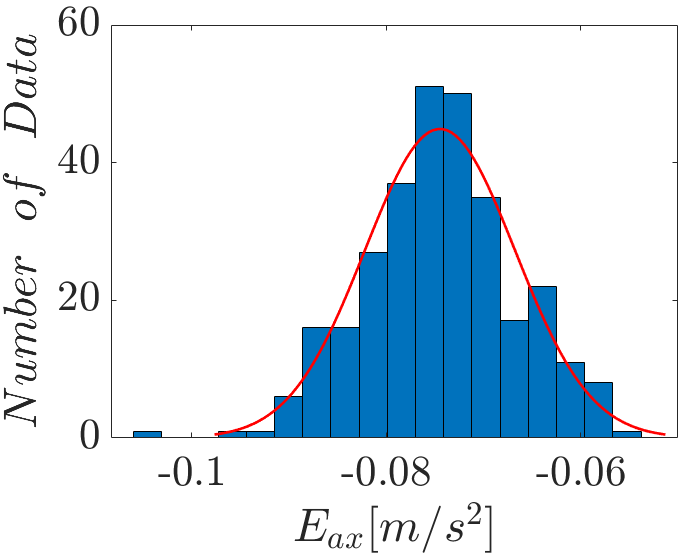
\includegraphics[width=0.235\textwidth]{curve/Eax.png}}
	\subfloat[Histogram of $Eay$]{\label{b}
	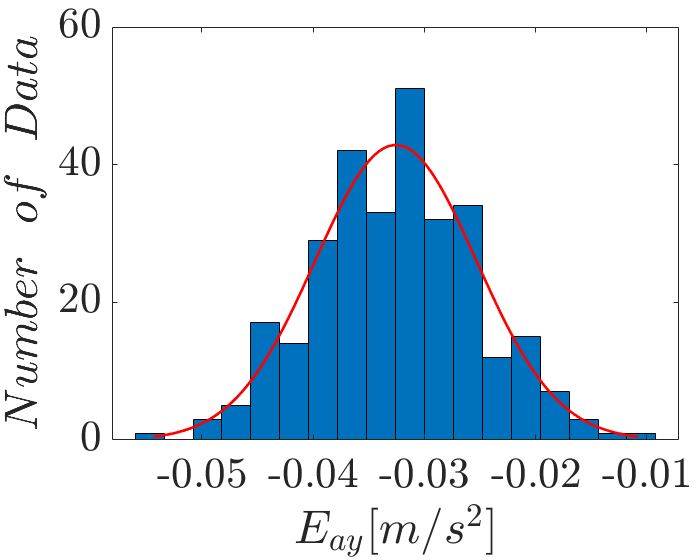
\includegraphics[width=0.235\textwidth]{curve/Eay.png}}  \\
	\subfloat[Histogram of $Eaz$]{\label{c}
	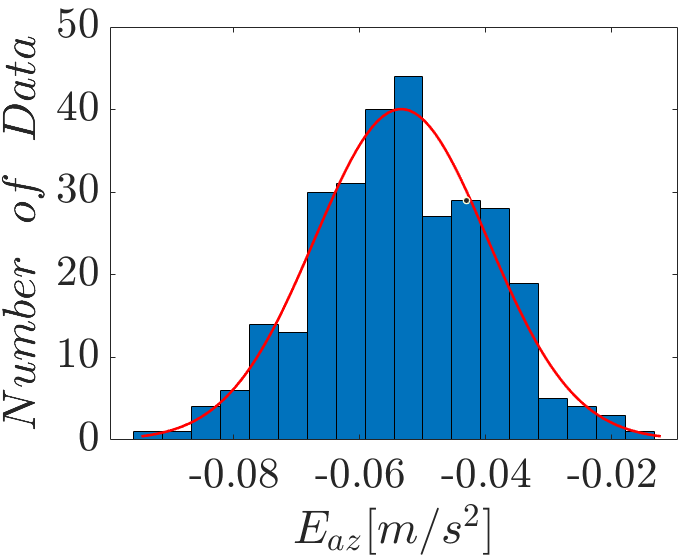
\includegraphics[width=0.235\textwidth]{curve/Eaz.png}}
	\subfloat[Histogram of $Ewx$]{\label{d}
	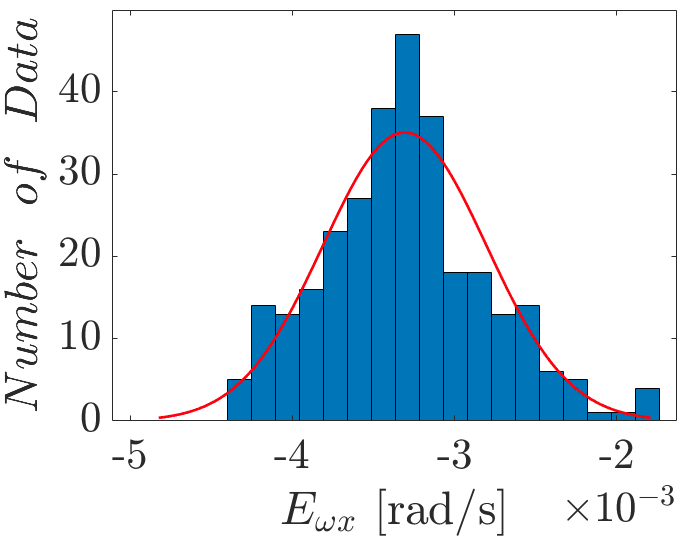
\includegraphics[width=0.235\textwidth]{curve/Ewx.png}}  \\
	\subfloat[Histogram of $Ewy$]{\label{e}
	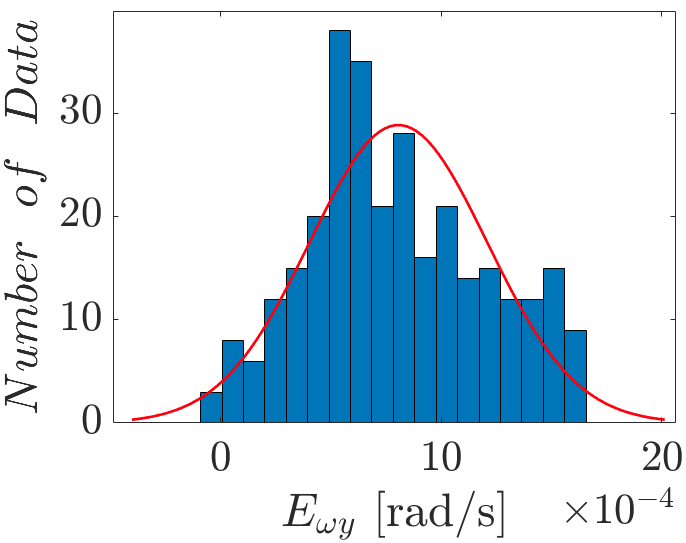
\includegraphics[width=0.235\textwidth]{curve/Ewy.png}}  
	\subfloat[Histogram of $Ewz$]{\label{f}
	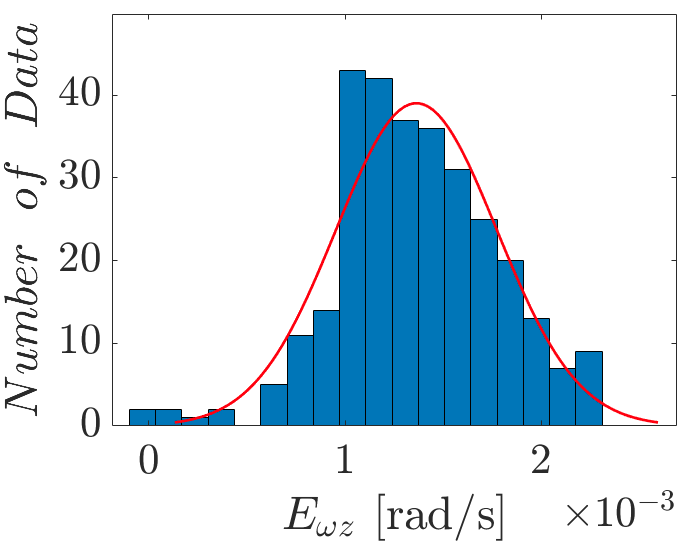
\includegraphics[width=0.235\textwidth]{curve/Ewz.png}}
	\centering
	\caption{Histogram of accelerometer and gyroscope sensor errors. Red curves are Gaussians with standard deviation fit to the data.}
	\label{Acceleration error histogram}
\end{figure}


\newpage
\subsection{Estimation Results}
\subsubsection{Results without Bias Estimation }
In the first measurement model, we integrate the velocity measurements in $x$ and $y$ directions and use the position measurements $(x,y,z)$ for the correction step. In the other measurement model, we process the range sensor data and use velocity measurements $(v_x,v_y,v_z)$ for the correction step. 

\begin{figure}[ht]
	\centering
	\subfloat[Estimated results for position $x$]{
	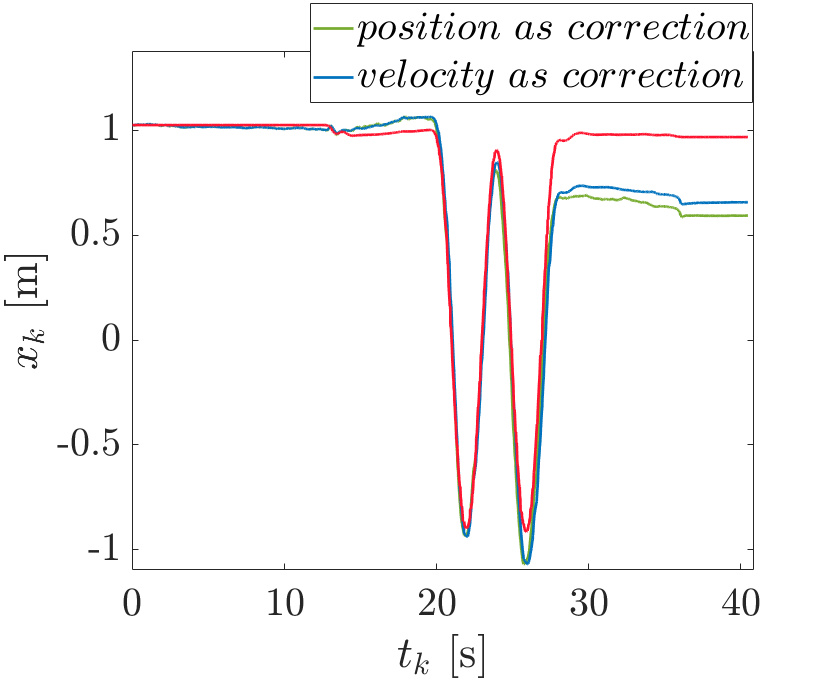
\includegraphics[width=0.235\textwidth]{curve/Tracking_x.png}\label{a}}
	\subfloat[Estimated results for position $y$]{\label{b}
	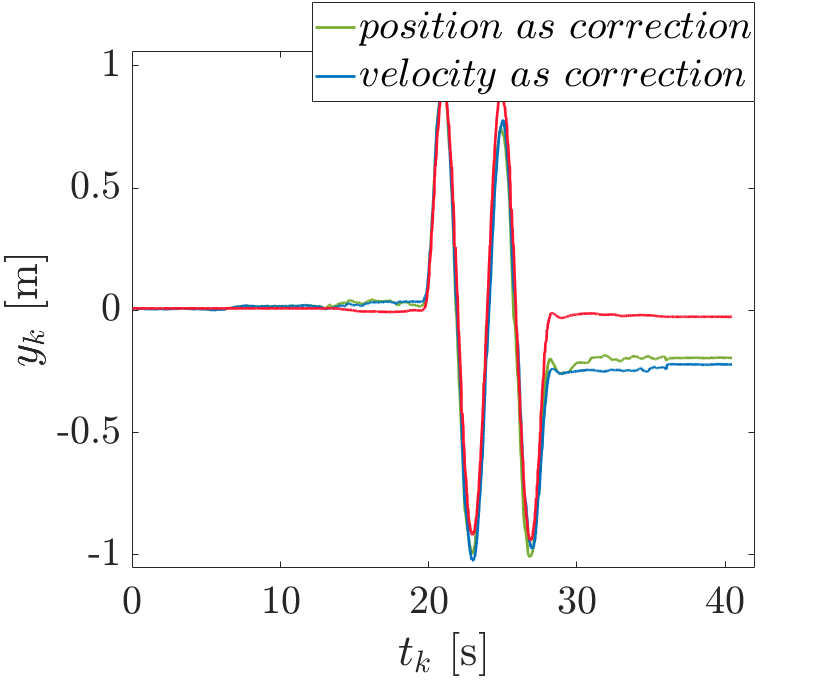
\includegraphics[width=0.235\textwidth]{curve/Tracking_y.png}}  \\
	\subfloat[Estimated results for position $z$]{\label{c}
	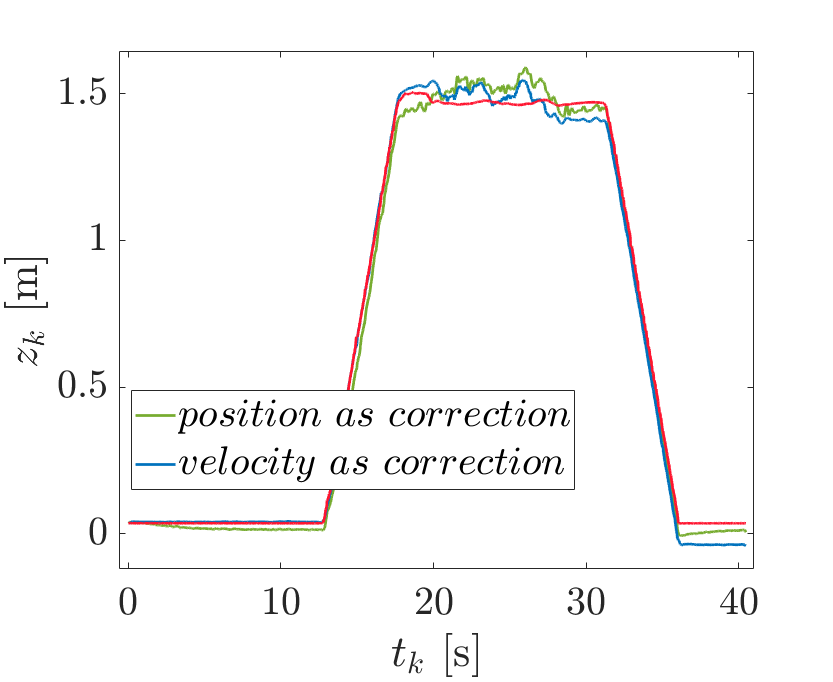
\includegraphics[width=0.235\textwidth]{curve/Tracking_z.png}}
	\subfloat[Estimated results for position $v_x$]{\label{d}
	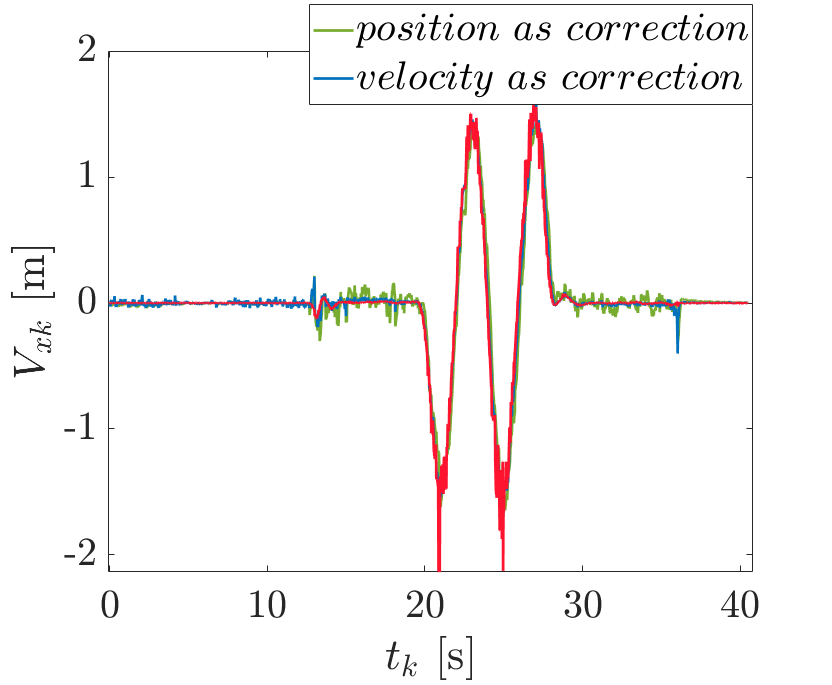
\includegraphics[width=0.235\textwidth]{curve/Tracking_vx.png}}  \\
	\subfloat[Estimated results for position $v_y$]{\label{e}
	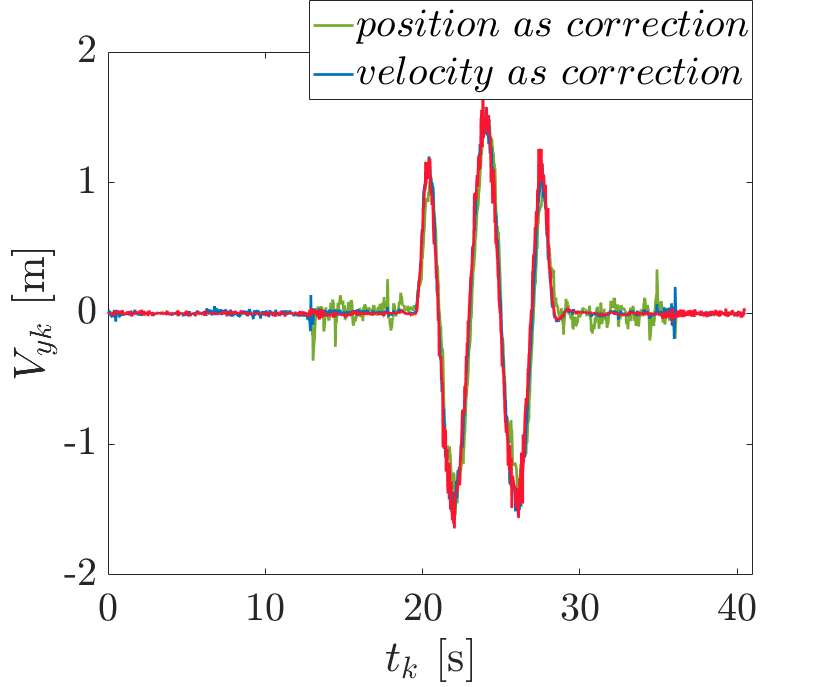
\includegraphics[width=0.235\textwidth]{curve/Tracking_vy.png}}
	\subfloat[Estimated results for position $v_z$]{\label{f}
	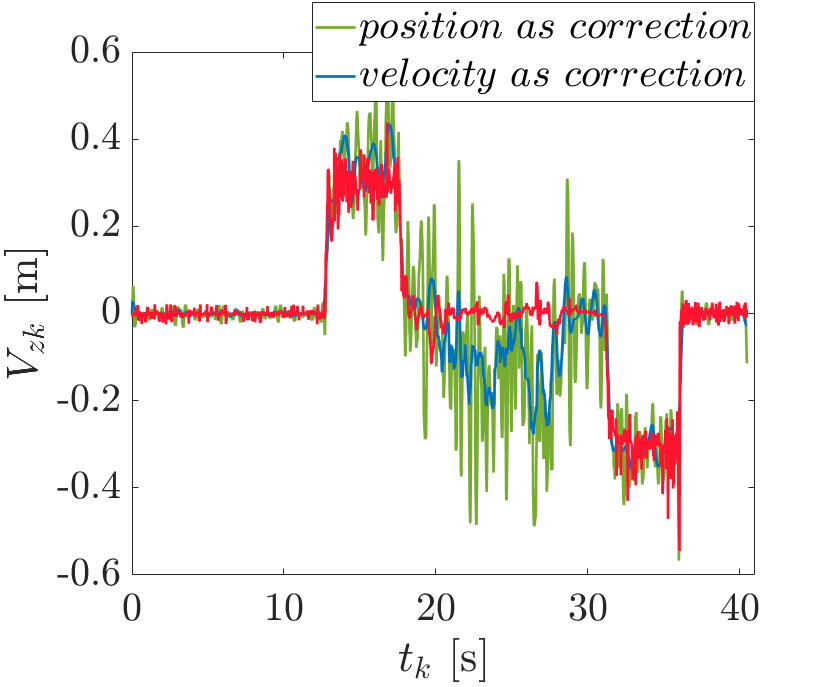
\includegraphics[width=0.235\textwidth]{curve/Tracking_vz.png}}
	\centering
	\caption{Estimation results of Crazyflie's position and velocity with different measurement models. The red curves are groundtruth values provided from Vicon system}
	\label{trackingfigure}
\end{figure}

Comparing with the groundtruth data, both measurement model provides a generally good estimation results (Fig.~\ref{trackingfigure}). However, the errors in position are slightly accumulated through the estimation process leading to slightly drifted estimation results. In $x$, $y$ and $z$ directions, the drifted errors are around $0.35$, $0.2$ and $0.05$ meters respectively. There are two major reasons leading to these drifted estimation results. First, as observed in the sensor data, both accelerometer and gyroscope provide biased sensor data. These biases will propagate and accumulate through out the estimation process and cause the drifted results. The second reason is that without direct correction for roll, pitch and yaw angles, the uncertainty of orientation affects the position.
 
From the estimation error plots in Fig.~\ref{errorfigure}, it could be observed that the first measurement model provides better estimation results in position states while the second model perform better in velocity states estimation. This phenomenon matches the intuition that with direct measurement data for correction, filter can provide better estimation results.

\begin{figure}[ht!]
	\centering
	\subfloat[Estimation error $E_x$]{\label{a}
	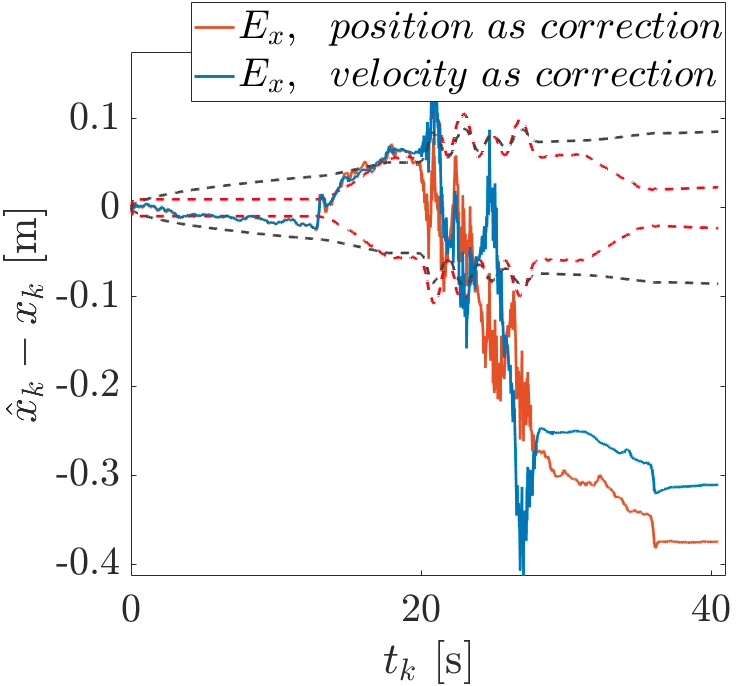
\includegraphics[width=0.235\textwidth]{curve/Error_x.png}}
	\subfloat[Estimation error $E_y$]{\label{b}
	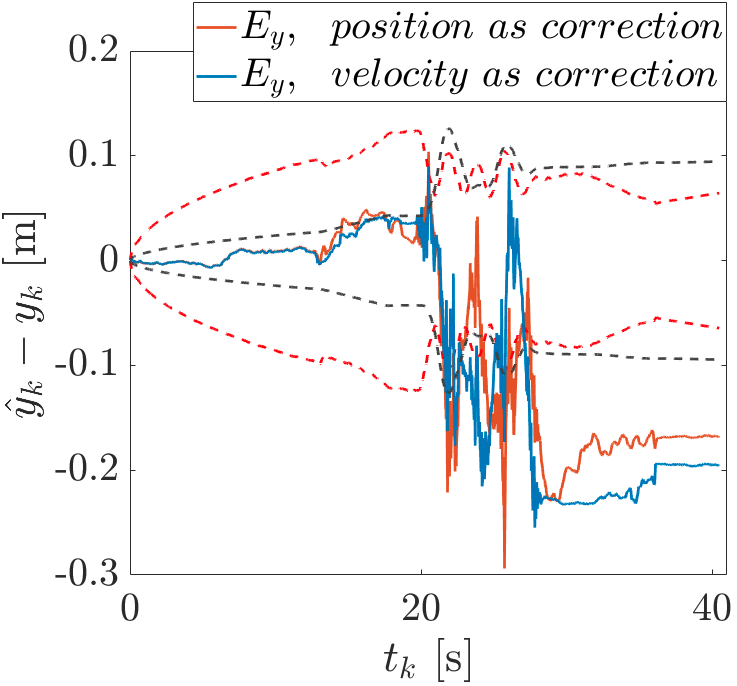
\includegraphics[width=0.235\textwidth]{curve/Error_y.png}} \\
	\subfloat[Estimation error $E_z$]{\label{c}
	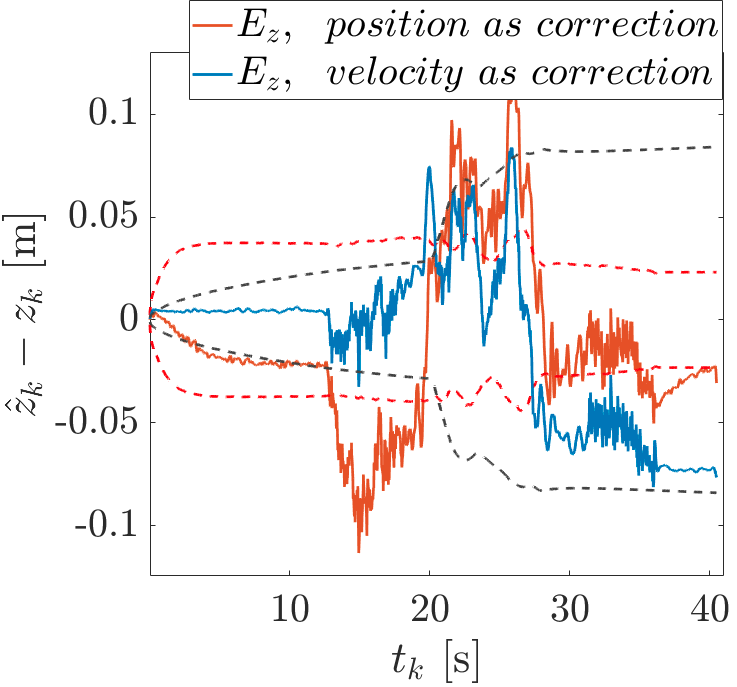
\includegraphics[width=0.235\textwidth]{curve/Error_z.png}}   
	\subfloat[Estimation error $E_{vx}$]{\label{d}
	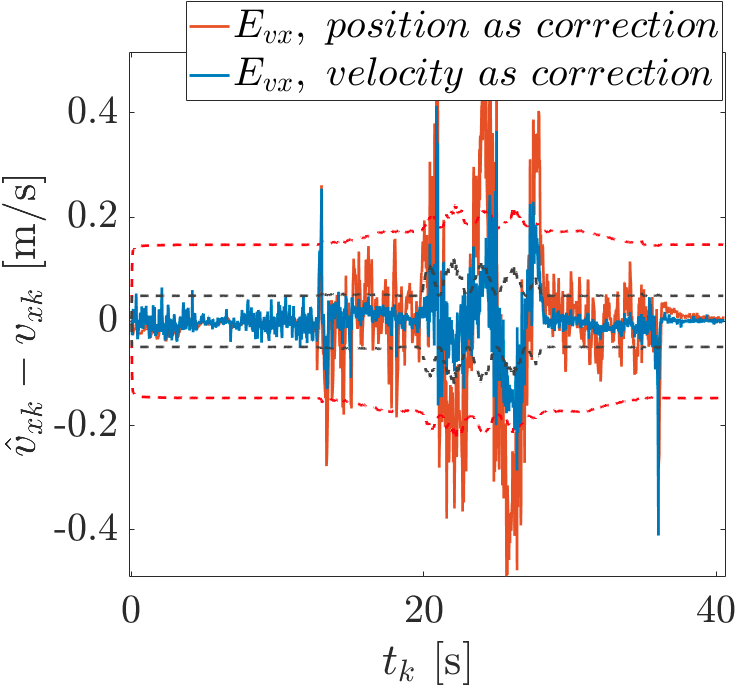
\includegraphics[width=0.235\textwidth]{curve/Error_vx.png}}  \\
	\subfloat[Estimation error $E_{vy}$]{\label{e}
	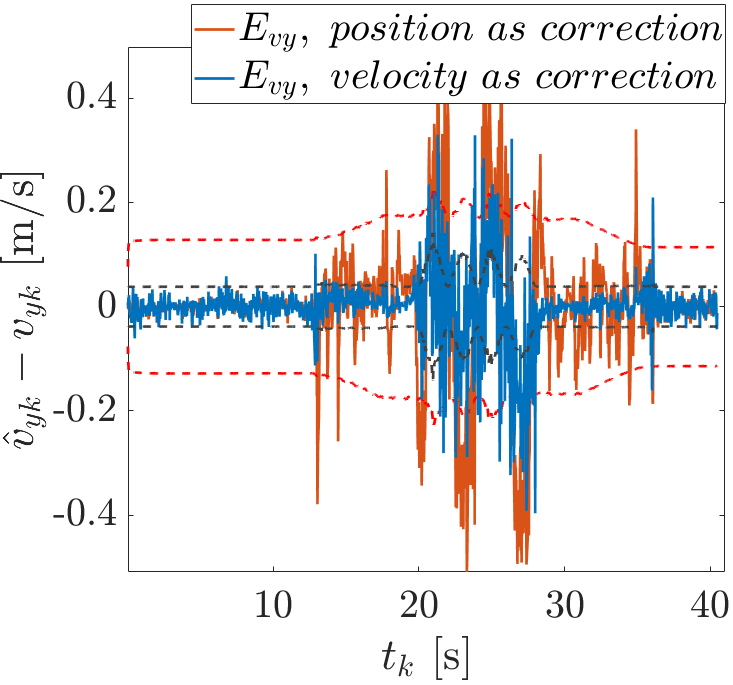
\includegraphics[width=0.235\textwidth]{curve/Error_vy.png}}  
	\subfloat[Estimation error $E_{vz}$]{\label{f}
	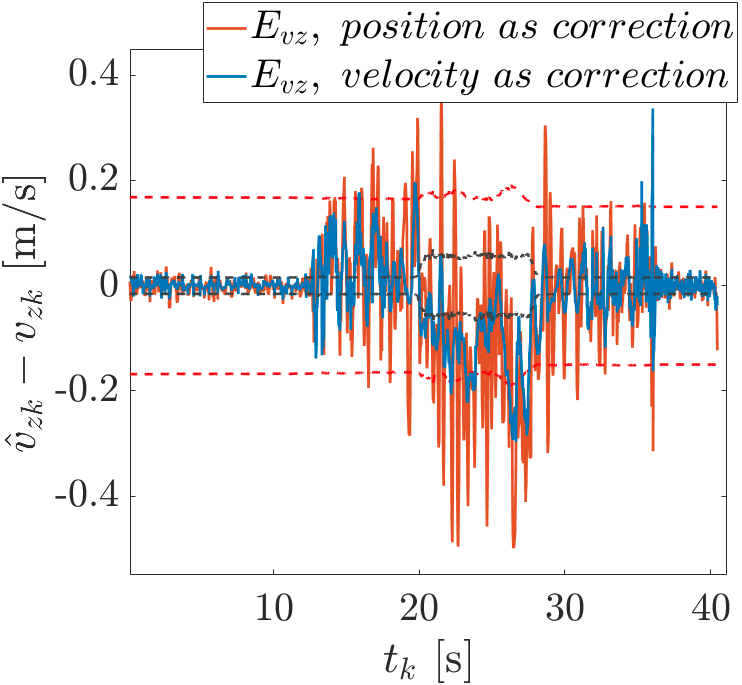
\includegraphics[width=0.235\textwidth]{curve/Error_vz.png}}
	\centering
	\caption{The estimation errors of Crazyflie's position and velocity with different measurement models campared with groundtruth data. The red and green dot curves are the $\pm3\sigma$ bands of the two models.}
      \label{errorfigure}
\end{figure}

\subsubsection{Results with Bias Estimation }
In bias estimation, we add the accelerometer and gyroscope sensor biases into estimator states and use the position measurements for correction. Comparing with this estimation results with the one in Fig.~\ref{errorfigure}, all the position and velocity estimation results are improved. From the plots in Fig.~\ref{biasfigure}, we can observe that the error of position $y$ estimation results decreases greatly from $0.2$ meters to around $0.05$ meters at the last time step. For the estimation of position $x$ and $z$, bias estimation also improves the estimator's performance. But due to the observability limitation, estimation result for position $x$ is still drifted. The bias estimation also improves the velocity states estimation during the flight. Totally, we can achieve more accurate position and velocity estimation results with sensor bias estimation which is essential for an autonomous safe landing.   

\begin{figure}%[ht]
	\centering
	\subfloat[Estimation error $E_x$]{\label{a}
	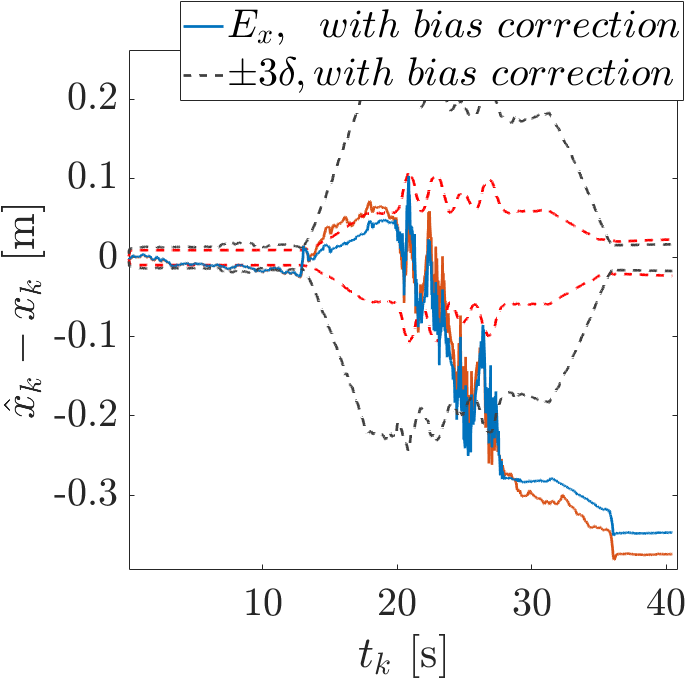
\includegraphics[width=0.235\textwidth]{curve/Bias_Ex.png}}
	\subfloat[Estimation error $E_y$]{\label{b}
	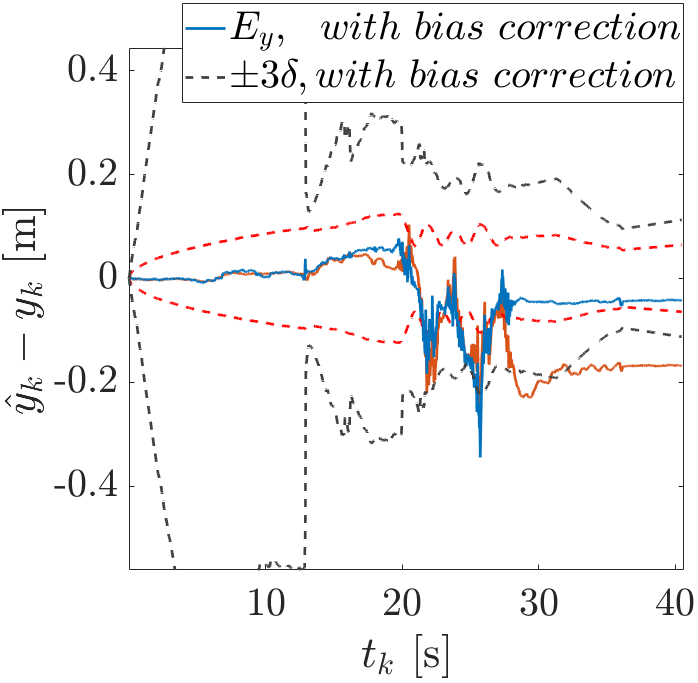
\includegraphics[width=0.235\textwidth]{curve/Bias_Ey.png} } \\
	\subfloat[Estimation error $E_z$]{\label{c}
	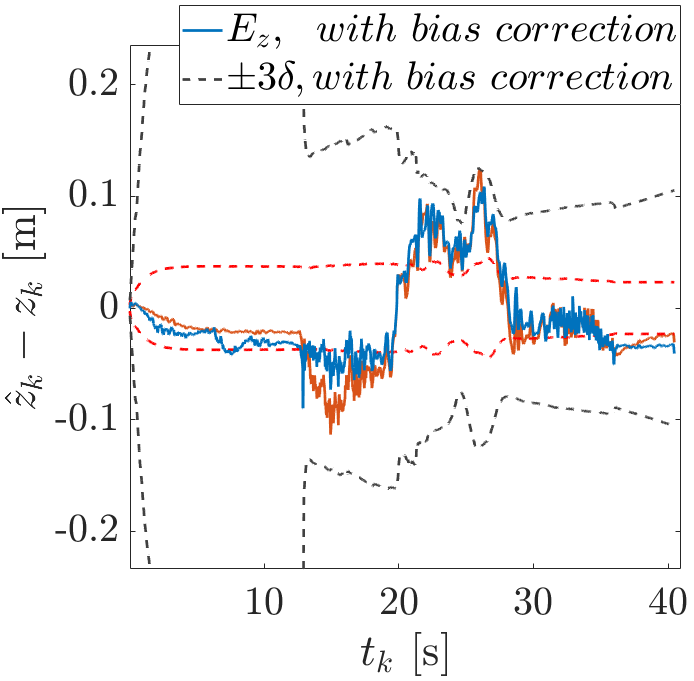
\includegraphics[width=0.235\textwidth]{curve/Bias_Ez.png}}
	\subfloat[Estimation error $E_{vx}$]{\label{d}
	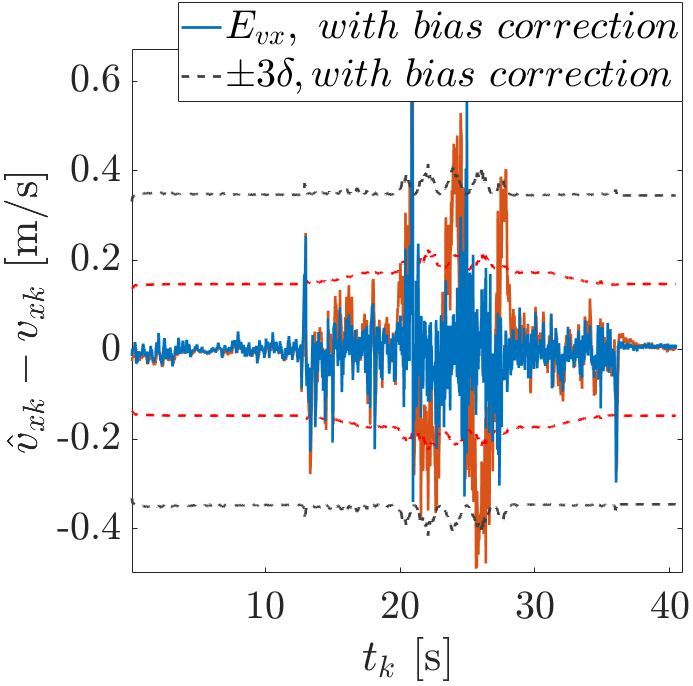
\includegraphics[width=0.235\textwidth]{curve/Bias_Evx.png}}  \\
	\subfloat[Estimation error $E_{vy}$]{\label{e}
	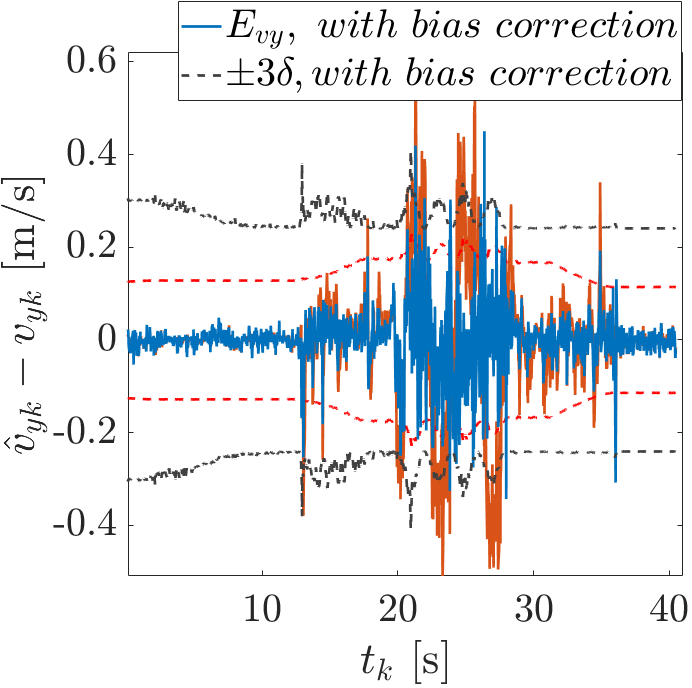
\includegraphics[width=0.235\textwidth]{curve/Bias_Evy.png}}
	\subfloat[Estimation error $E_{vz}$]{\label{f}
	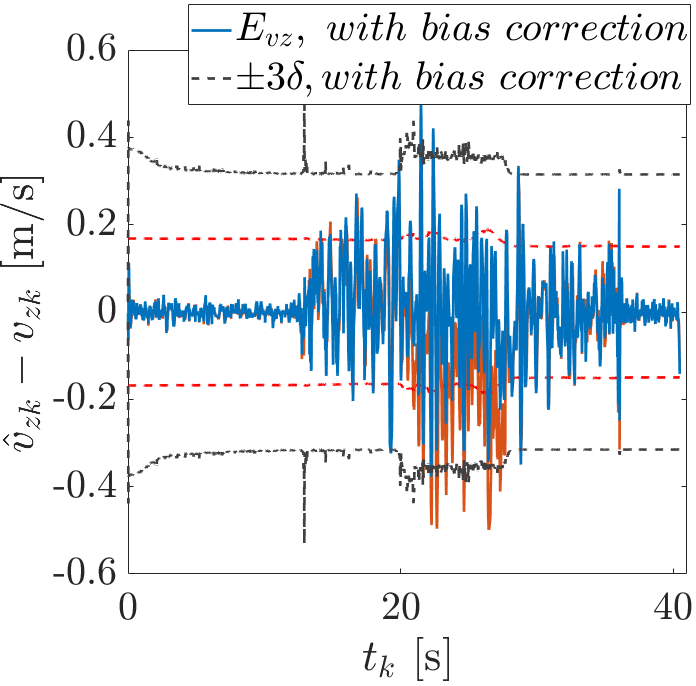
\includegraphics[width=0.235\textwidth]{curve/Bias_Evz.png}}
	\centering
	\caption{The estimation errors comparison of Crazyflie's position and velocity with and without bias states. The blue curves indicate the estimation errors with bias states and the green dot lines are their corresponding $\pm3\sigma$ bands.}
      \label{biasfigure}
\end{figure}

\section{CONCLUSION AND FUTURE WORK}

The Extended Kalman Filter for estimating the position, velocity and orientation of a quadrotor with onboard IMU and flow deck sensor were implemented in this work. Different measurement models are used for correction step and the limitation of the estimator is discussed through observability analysis. 

In order to achieve more accurate estimation results, we added bias estimation and correction into our work. The estimated results for position and velocity are greatly improved with bias correction, especially in positions $y$ and $z$. However, due to observability constraints, the estimation result of position $x$ still shows error about $0.35$ meters.

As future work, we will investigate adding more sensors onboard which could provide more measurement information in order to improve the performance of the estimator. The final goal is to design a motion planning and control algorithm for emergency landing scenarios. In addition, we aim to extend our work into a swarm of quadrotors for multi-agent emergency landing.      

\addtolength{\textheight}{-12cm}   % This command serves to balance the column lengths



\nocite{*}

\bibliographystyle{IEEEtran}
\bibliography{ref.bib}



\end{document}